\section{Personas}\label{l:personas}

\begin{table}
\begin{center}
\begin{tabular}{@{}l l}
\textbf{Projektleiter} &\\

\hline \\ [-1ex]

Arthur Blozyk & \emph{Sales Information and Communication}\\ 
\emph{Dipl. Ingenieur, Dipl. Wirtschaftsingenieur} & \trademark{MAN Truck \& Bus AG}\\[1ex]

Sebastian Nell & \emph{Director of USE // Connected Products}\\
& \trademark{Scholz \& Volkmer GmbH}\\[1ex]

Tobias Rudolphi	& \emph{Lead Software Architect}\\
\emph{Dipl. Informatik} & \trademark{Zühlke Engineering GmbH}\\[2ex]

\textbf{Konzept, Design} &\\

\hline \\ [-1ex]

Carsten Fischer	& \emph{UX Designer \& Informationsarchitekt}\\
\emph{M.A. Sozialwissenschaften, Anglistik} & \trademark{triplesense GmbH}\\[1ex]

Eva Kümml & \emph{Senior Konzept / User Experience}\\
\emph{Dipl. Medienwirtin} & \trademark{SinnerSchrader Deutschland GmbH}\\[1ex]

Sandra-Charlotte Hildebrandt & freie Art-Direktorin\\
\emph{Dipl. Designerin} &\\[2ex]

\textbf{Produktion} &\\

\hline \\ [-1ex]

Sebastian Beyer	& \emph{Developer}\\
\emph{Informatik, B.Sc.} & \trademark{Scholz \& Volkmer GmbH}\\[1ex]

Jan Lochner	& Freelancer\\
\emph{Dipl. Multimedia Producer} & \\[2ex]

\textbf{Texter} &\\

\hline \\ [-1ex]

Marc Stenzel & Fachjournalist, freier Projektleiter\\[1ex]

Torsten Schölzel & freier Texter\\
\emph{Dipl. Soziologe} & \\[2ex]

\textbf{Übersetzer} &\\

\hline \\ [-1ex]

Jorinde Gessner	& \emph{Information Manager}\\
\emph{German and Politics, B.A. Hons} & \trademark{Ogilvy \& Mather Deutschland GmbH}\\[2ex]

\textbf{Kunde} &\\

\hline \\ [-1ex]

Markus Rüb & \emph{Sales Information and Communication}\\
\emph{Dipl. Wirtschaftsingenieurwesen} & \trademark{MAN Truck \& Bus AG}

\end{tabular}
\caption{Interviewte Personen}
\label{table:interviewpartner}
\end{center}
\end{table}

Im vorigen Abschnitt wurden die Probleme geschildert, die in Projekten auftreten, in denen Informations- und Kommunikationsmedien erstellt werden und daraus gefolgert, welches die wichtigsten Aspekte sind, die eine mögliche Lösung berücksichtigen muss. In diesem Abschnitt werden Personas vorgestellt, die die typischen Benutzergruppen des Systems repräsentieren und ihre Aufgaben und Erwartungen zusammengefasst. 

\begin{quote}
\citequotes{Personas describe a site’s target users, giving a clear picture of how they’re likely to use the system, and what they’ll expect from it, among other things. […] Without personas, there is no common language for talking about what users want.} \cite[S.15 ff.]{brown2007communicating}
\end{quote}

Personas sind ein wichtiger Baustein für die Konzeption eines Systems. Sie ermöglichen es, Bestandteile des Konzepts schon während des Entwurfs zu verifizieren, in dem deren Auswirkungen mit dem Nutzungsverhalten und den Erwartungen der Personas verglichen werden. Personas bilden nicht nur im Konzept eine wichtige Entscheidungshilfe sondern werden auch während des Entwurfs und der Umsetzung immer wieder zu Rate gezogen, in dem Funktionalitäten auf deren Relevanz und mögliche Probleme für bestimmte Personas hin überprüft werden. \cite[S.38 ff.]{cohn2004user}

Die Personas basieren auf im April 2012 geführten Interviews mit den in Tabelle~\ref{table:interviewpartner}~(S.\pageref{table:interviewpartner}) aufgezählten Personen. Die Namen und Fotos der Personas basieren zwar auf den interviewten Personen, dienen aber lediglich dazu, das Merken der Personas zu erleichtern. 

\begin{figure}[htb]
\begin{center}
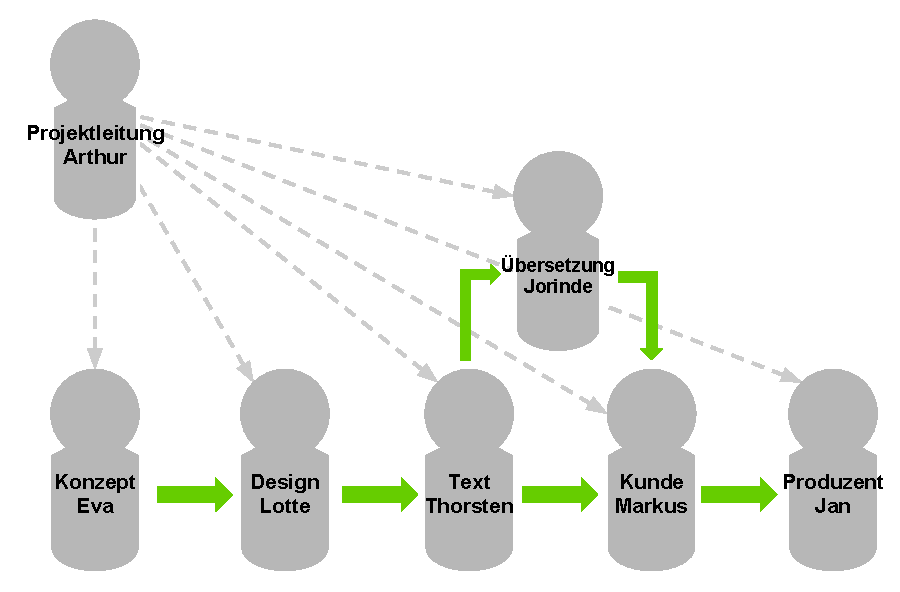
\includegraphics[width=\textwidth]{media/Uebersicht-Personas.pdf}
\caption{Übersicht über die Personas und den idealisierten Workflow}
\label{chart:uebersicht-personas}
\end{center}
\end{figure}

Die Auswahl der Personas orientiert sich an dem vorherrschenden Workflow innerhalb der Projekte. Wie in Abschnitt~\ref{l:problemanalyse}~(S.\pageref{l:problemanalyse}) gezeigt wurde, gibt es in der Praxis keinen linearen Ablauf, sondern es ergeben sich vielzählige Feedback-Schleifen. Vernachlässigt man diese Feedback- und Korrekturschleifen kann man die beteiligten Personen in eine, in Abbildung~\ref{chart:uebersicht-personas}~(S.\pageref{chart:uebersicht-personas}) gezeigte, lineare Reihenfolge bringen:
\begin{samepage}\begin{enumerate}\itemsep -5pt
\item Konzepterin \emph{Eva} entwickelt das Produkt, wobei sie die Rahmenbedingungen wie Aufbau, Umfang, Zielgruppe, Ansprache festlegt. 
\item Designerin \emph{Lotte} gestaltet das Produkt, wobei sie bestimmt, wie Texte dargestellt werden (Satz, Länge, Schriftart, Farben, Hervorhebungen)
\item Texter \emph{Torsten} erstellt die Texte für das Produkt in der Ausgangssprache
\item Kunde \emph{Markus} nimmt die Texte ab
\item Übersetzerin \emph{Jorinde} übersetzt die Texte
\item Produzent \emph{Jan} übernimmt die Texte in das Produkt
\end{enumerate}\end{samepage}

Eine wichtige Rolle fehlt in dieser Auflistung: Projektleiter \emph{Arthur} koordiniert den Ablauf des Projektes, hat aber keinen Einfluss den Text. Er darf jedoch als wichtiges Bindeglied zwischen allen Beteiligten  nicht fehlen.

Bei der Formulierung der Personas wurde bewusst darauf verzichtet, persönliche Daten wie Alter und Bildung zu verwenden, da diese keinen Einfluss auf die Konzeption des Systems haben. Die Personas enthalten dementsprechend nur 
\begin{itemize}\itemsep -5pt
\item den wichtigsten Nutzen aus der Sicht der Person als Zitat
\item eine Beschreibung der Aufgabe der Rolle, die diese Persona repräsentiert
\item Angaben zu den Beteiligten, mit denen sich die Person im Verlauf des Projektes \emph{über Texte} austauschen wird
\item die verwendeten Werkzeug zur Erfüllung der Aufgabe und die Erfahrung im Umgang mit Anwendungen im Allgemeinen
\item die wichtigsten Szenarien, die die Persona mit Hilfe des Systems durchführen wird
\item allgemeine Anforderungen an das System
\item und Angaben darüber, wie der Zugriff auf das System erfolgt.
\end{itemize}

Diese Information bilden die Basis für die Konzeption einer browserbasierten Web-Anwendung im Abschnitt~\ref{l:konzeption}~(S.\pageref{l:konzeption}).

% PERSONAS

\pagebreak

\subsection{\emph{Eva}, Konzepterin}\label{p:eva}

\begin{multicols}{2}

\begin{center}
\fbox{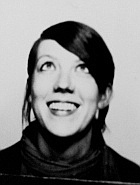
\includegraphics[width=0.5\columnwidth]{media/eva.jpg}}
\end{center}

\citequotes{Ich möchte, dass alle Beteiligten einen guten Überblick über das Produkt haben.}

Eva konzipiert als Informationsarchitektin das Produkt. Dabei legt sie entsprechend der Zielsetzung fest, wie das Produkt aufgebaut ist um die Erwartungen des Nutzers zu erfüllen und ihn das gewünschten Ergebnis im Sinne des Produktes leicht erreichen zu lassen. Hierzu erstellt sie einen Überblick über das Produkt mit Hilfe von Wireframes und macht dabei Vorgaben über die Platzierung von Texten und deren Funktion.

\textbf{Organisation, Abstimmung}

Eva arbeitet auf Seite der Agentur und stimmt sich mit \emph{Markus}~(\ref{p:markus}) sowie \emph{Lotte}~(\ref{p:lotte}) über das Produkt ab. Sie gibt Feedback zu den Texten von \emph{Torsten}~(\ref{p:torsten}) und deren Integration in das Produkt durch \emph{Jan}~(\ref{p:jan}).

\textbf{Werkzeuge und Erfahrung}

Evas wichtigstes Werkzeug ist \trademark{OmniGraffle} von \trademark{Omni Group} mit dem sie die Wireframes des Produktes erstellt. Sie ist versiert im Umgang mit vielfältigen Anwendung und steht neuen Werkzeugen offen gegenüber.

\columnbreak

\textbf{Szenarien}

Eva definiert die einzelnen logischen Bestandteile des Produktes (z.B. Seiten, Abschnitte) und definiert darin, welche einzelnen Textbausteine verwendet werden.

Eva legt Rahmenbedingungen für den Text fest. Zum einen bestimmt sie die Ansprache, d.h. welche Zielgruppe soll mit den Texten angesprochen werden und welches Ziel verfolgen die Nutzer. Zum anderen macht sie Vorgaben über den Aufbau einzelner Klassen von Texten wie z.B. Überschriften, Schaltflächen, Fließtext bei denen sie z.B. die Textlänge, Spaltenbreite oder Zeilenanzahl festlegt. Diese Rahmenbedingungen kann sie zu den jeweiligen Textbausteinen hinterlegen.

Eva kann sich eine Übersicht ausdrucken, die alle Bestandteile des Produktes enthält. So kann sie leicht den Überblick behalten.

\textbf{Anforderungen}

Eva verwendet das System häufig, deswegen müssen Funktionen zur Definition des Produktes, der Texte und der Rahmenbedingungen einfach zu bedienen sein. Sie will nie die Übersicht verlieren und leicht Elemente verändern können, da sich in der Konzeptionsphase häufig Änderungen ergeben. 

\textbf{Zugang}

Eva greift auf das System mit ihrem \trademark{MacBook Pro} zu, sie verfügt über einen zusätzlichen großen Bildschirm und eine schnelle Internetverbindung.

\end{multicols}

\pagebreak

\subsection{\emph{Lotte}, Designerin}\label{p:lotte}

\begin{multicols}{2}

\begin{center}
\fbox{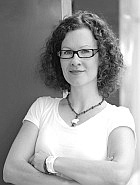
\includegraphics[width=0.5\columnwidth]{media/lotte.jpg}}
\end{center}

\citequotes{Ich möchte, dass meine Vorgaben zur Gestaltung der Texte von allen berücksichtigt werden.}

Lotte gestaltet als Art-Direktorin das Produkt. Sie entwirft dazu das Fein-Layout auf Basis der Wireframes, die von \emph{Eva}~(\ref{p:eva}) erstellt wurden, indem sie für alle Darstellungs-Varianten präzise Entwürfe anfertigt. Hierbei legt sie auch genaue Vorgaben für die Formatierung der Texte im Produkt fest.

\textbf{Organisation, Abstimmung}

Lotte arbeitet auf Seiten der Agentur und stimmt sich mit \emph{Eva}~(\ref{p:eva}) bei der Gestaltung des Produktes ab. Mit \emph{Torsten}~(\ref{p:torsten}) spricht sie über ihre Vorgaben zu Texten und überprüft deren Einhaltung in der Umsetzung durch \emph{Jan}~(\ref{p:jan}).

\textbf{Werkzeuge und Erfahrung}

Lotte arbeitet mit den Produkten der \trademark{Adobe Creative Suite}. Sie ist nur im Umgang mit wenigen anderen Werkzeugen versiert, steht neuen Anwendungen aber offen gegenüber.

\textbf{Zugang}

Lotte greift auf das System mit ihrem \trademark{iMac} zu, sie verfügt über einen großen Bildschirm und eine schnelle Internetverbindung.

\columnbreak

\textbf{Szenarien}

Lotte erstellt einen Styleguide und legt dabei fest, welche Text-Klassen im Produkt verwendet werden. Text-Klassen sind z.B. Überschriften, Untertitel und Fließtext. Dazu macht sie für jede Klasse Angaben zu der verwendeten Schriftart, die Einschränkungen, wie z.B. die maximalen Zeilenanzahl oder Menge der Zeichen pro Zeile.

Lotte erstellt Layouts in Form von Screenshots oder Beispielseiten. Hierbei verwendet Sie für die Texte die noch nicht durch \emph{Eva}~(\ref{p:eva}) festgelegt wurden, Blindtexte. Um ein besseres Gefühl für die Inhalte zu bekommen und die Layouts besser mit dem Kunden abstimmen zu können möchte Lotte gerne jetzt schon einige Texte von \emph{Torsten}~(\ref{p:torsten}) in den Layouts verwenden.

Während der Umsetzung des Produktes ergeben sich Änderungen am Styleguide. Sie möchte, dass \emph{Jan}~(\ref{p:jan}) alle Stellen im Produkt anpasst, die von dieser Änderungen betroffen sind.

\textbf{Anforderungen}

Lotte möchte das Anlegen von Text-Vorgaben unkompliziert und schnell erledigen können. Änderungen müssen jederzeit und ohne großen Aufwand möglich sein. Das System muss leicht verständlich sein, da sie nie viel Zeit damit verbringt. Komplizierte Abläufe würden Sie abschrecken und sie würde statt dessen eine E-Mail schreiben.

Lotte hat sehr hohe Ansprüche an die Gestaltung des Systems.

\end{multicols}

\pagebreak

\subsection{\emph{Torsten}, Texter}\label{p:torsten}

\begin{multicols}{2}

\begin{center}
\fbox{
\includegraphics[width=0.5\columnwidth]{media/torsten.jpg}}
\end{center}

\citequotes{Ich möchte den Texteditor an meine Bedürfnisse anpassen können und beim Schreiben in meinem \typoquotes{Flow} nicht unterbrochen werden.}

Torsten erstellt auf Basis der vom Kunden gelieferten Materialien oder bereits bestehender Produkte die Texte für das Produkt. Hierbei muss er Vorgaben aus dem Konzept und dem Design berücksichtigen, sowie Wünschen und möglicherweise verbindliche Richtlinien des Kunden beachten. Hierzu erstellt Torsten für alle Textbausteine des Produktes die Texte in der endgültigen Fassung in seiner Muttersprache.

\textbf{Organisation, Abstimmung}

Torsten ist selbständig. Er stimmt sich mit \emph{Eva}~(\ref{p:eva}) und \emph{Lotte}~(\ref{p:lotte}) bezüglich deren Vorgaben ab. Er berücksichtigt inhaltliche Vorgaben, die er von \emph{Markus}~(\ref{p:markus}) erhält. Er steht  \emph{Jorinde}~(\ref{p:jorinde}) für Rückfragen zur Verfügung.

\textbf{Werkzeuge und Erfahrung}

Torsten arbeitet mit \trademark{iWorks Pages} von \trademark{Apple}, da er die vielen Funktionen von \trademark{Word} als störend empfindet und diese nicht benötigt. Er ist nur im Umgang mit wenigen Programmen vertraut.

\columnbreak

\textbf{Szenarien}

Torsten verfasst die Texten zum Produkt, dazu befüllt der die vom Design vorgegeben Textbaustein. Dabei bekommt kann er die Vorgaben sehen, die für den jeweiligen Text gelten (z.B. maximale Textlänge). 

Torsten benötigt Kontext-Information zum aktuellen Text und kann im System die vom Kunden zur Verfügung gestellten Materialien aufrufen. Auch die Hinweise zur Zielgruppe und Funktion des Textes aus dem Konzept kann er sich ansehen, ohne die aktuelle Ansicht des Systems verlassen zu müssen.

Der Kunde wünscht Änderungen an den Texten. Diese sind im System bei den jeweiligen Textbausteinen hinterlegt, so das Torsten die Texte schnell anpassen kann, ohne sie erst aufwändig suchen zu müssen.

Torsten arbeitet in einem Team mit anderen Textern und führt die Qualitätskontrolle an den Texten seiner Kollegen durch.

\textbf{Anforderungen}

Das Editor zum Erstellen von Texten muss im System an Torsten Bedürfnisse anpassbar sein. Er möchte genaue Kontrolle darüber haben, \emph{wann} andere Projektmitarbeiter seine Texte sehen können. Feedback zu Texten soll zu den jeweiligen Textbausteinen zugeordnet werden können.

\textbf{Zugang}

Torsten arbeitet in seinem eigenen Büro oder von unterwegs, da er an mehreren Projekten gleichzeitig arbeitet. Er greift auf das System mit seinem \trademark{MacBook Pro} zu und je nach Standort kann seine Internetverbindung auch nur mittel schnell sein.

\end{multicols}

\pagebreak

\subsection{\emph{Markus}, Kunde}\label{p:markus}

\begin{multicols}{2}

\begin{center}
\fbox{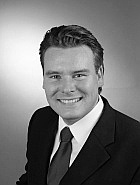
\includegraphics[width=0.5\columnwidth]{media/markus.jpg}}
\end{center}

\citequotes{Ich möchte, dass die Vorgaben aus unserer Marketing"~, Fach"~ und Rechtsabteilung genau berücksichtigt werden. Änderungswünsche und Korrekturen sollen exakt befolgt werden.}

Markus ist der Auftraggeber des Produktes. Er ist der erste Ansprechpartner für die Agentur, steht aber auch stellvertretend für weitere Unternehmensmitarbeiter aus verschiedenen Abteilungen seines Unternehmens. Er liefert Materialien und Vorgaben die als Basis für die zu erstellenden Texte dienen. Er führt auch die finale Abnahme der Texte und des Produktes durch.

\textbf{Organisation, Abstimmung}

Markus stimmt sich über den Zweck des Produktes mit \emph{Eva}~(\ref{p:eva}) ab. \emph{Torsten}~(\ref{p:torsten}) gibt er Feedback und Änderungswünschen zu dessen Texten. Auch die Übersetzungen von \emph{Jorinde}~(\ref{p:jorinde}) kontrolliert und verbessert er. Wurden die Texte in das Produkt übernommen, gibt er Änderungswünsche an den Inhalten und der Darstellung an \emph{Jan}~(\ref{p:jan}) weiter.

\textbf{Werkzeuge und Erfahrung}

Markus arbeitet vor allem mit \trademark{Word}, \trademark{Excel} und \trademark{PowerPoint}, ansonsten hat er keine weiteren Erfahrungen im Umgang mit Werkzeugen.

\columnbreak

\textbf{Szenarien}

Markus nimmt die fertigen Texte ab. Hierzu kann er einzelnen Textbausteine freigeben oder Änderungen anfordern, die er mit Hilfe von Kommentaren beschreibt. 

Um den Projektablauf nicht zu verzögern beantwortet Markus Rückfragen zu Texten von unterwegs.

Materialien können in das System eingestellt und einzelnen Textbausteinen oder ganzen Abschnitten zugeordnet werden.

Markus kann sich alle Texte als \trademark{Word}-Dokument exportieren um Korrekturen darin vorzunehmen. Anschließend importiert er das Dokument. Dabei werden die Änderungen automatisch im System übernommen.

\textbf{Anforderungen}

Das System \citequotes{muss einfach funktionieren}, da er nicht gezwungen werden will, ein neues System zu erlernen. Er erwartet, dass die wichtigen Funktionen auch mobil verfügbar sind. Die Daten im System und der Zugriff darauf müssen sicher sein. Er will festlegen, wer Zugriff erhält, mit der Möglichkeit, dies auch für einzelne Bereiche des Projektes definieren zu können.

\textbf{Zugang}

Markus arbeitet von seinem Büro-PC aus und greift auf das System mit einer schnellen Internetverbindung zu. Er ist viel unterwegs und verwendet dann sein \trademark{iPhone} oder seinen \trademark{iPad}.

\end{multicols}

\pagebreak

\subsection{\emph{Jorinde}, Übersetzerin}\label{p:jorinde}

\begin{multicols}{2}

\begin{center}
\fbox{
\includegraphics[width=0.5\columnwidth]{media/jorinde.jpg}}
\end{center}

\citequotes{Zum Übersetzen brauche ich eine praktische Darstellung der Original-Texte. Der Zugriff auf Kontext-Informationen muss leicht möglich sein.}

Jorinde übersetzt die Texte des Projektes in ihre Muttersprache. Sie berücksichtigt dabei bestehende Materialien des Kunden, sowie die Vorgaben aus Konzept und Design.

\textbf{Organisation, Abstimmung}

Jorinde arbeitet in einem Übersetzungsbüro als Teil eines Teams von Übersetzern, die das gesamte Projekt übersetzen. Sie stimmt sich mit \emph{Torsten}~(\ref{p:torsten}) bei inhaltlichen Fragen zu Texten ab. Für die Übersetzung spezieller Begriffe stimmt sie sich mit \emph{Markus}~(\ref{p:markus}) ab.

\textbf{Werkzeuge und Erfahrung}

Jorinde verwendet zum Erstellen der Übersetzung \trademark{Word}, da ihr dort Komfortfunktionen wie Rechtschreibkorrektur und Synonyme zur Verfügung stehen.  Jorinde hat wenig Erfahrung mit anderen Werkzeugen und braucht im allgemeinen länger, um sich an neue Systeme zu gewöhnen.

\textbf{Zugang}

Jorinde greift auf das System nur von ihrem Firmen-PC aus zu und verfügt über eine schnelle Internetverbindung.

\columnbreak

\textbf{Szenarien}

Jorinde übersetzt die Texte des Projekts, dazu werden die Originaltexte direkt in der Übersetzungsansicht dargestellt. Die Zusatzinformationen zu den Textbausteinen stehen ihr, wie bei \emph{Torsten}~(\ref{p:torsten}), in der Ansicht zur Verfügung.

Jorinde ist sich bei der Übersetzung eines bestimmten Begriffes unsicher. Sie verwendet das zur Verfügung gestellt Ausgangs-Material des Kunden um die Übersetzung nachzuschlagen, die in Publikationen des Kunden üblicherweise verwendet wird. Für zukünftige Verwendung hinterlegt sie dies im Glossar des Projektes.

Das Projekt enthält an mehreren Stellen die gleichen Formulierungen. Jorinde erhält an diesen Stellen die Übersetzung vorgeschlagen, die sie bereits angelegt hat. Sie kann diese direkt übernehmen oder eine Variante anlegen.

Jorinde sucht für einen Begriff ein Synonym. Sie kann sich direkt in der Ansicht zu dem Begriff Synonyme aus einem globalen Wörterbuch anzeigen lassen. Zusätzlich kann sie sich für das Wort in der Orginalsprache die Übersetzungen anzeigen lassen, die bereits im Projekt verwendet wurden.

Jorinde führt die Qualitätskontrolle an übersetzten Texten ihrer Kollegen durch.

\textbf{Anforderungen}

Jorinde benötigt zum Übersetzen im System die Hilfsmittel, die ihr auch in \trademark{Word} zur Verfügung stehen: Rechtschreibkorrektur, Synonyme sowie die nahtlose Integration von Wörterbüchern in mehreren Sprachen.

\end{multicols}

\pagebreak

\subsection{\emph{Jan}, Produzent}\label{p:jan}

\begin{multicols}{2}

\begin{center}
\fbox{
\includegraphics[width=0.5\columnwidth]{media/jan.jpg}}
\end{center}

\citequotes{Ich muss exakt wissen, welche Texte an welche Stelle im Produkt gehören. Bei Änderungen am Text möchte ich nicht jedes mal die Texte per Copy\&Paste übertragen müssen.}

Jan ist für die Erstellung des Produktes verwantwortlich. Er hat aber auch während der Entwurfsphase Einfluss auf die Rahmenbedingungen für Texte, vor allem wenn es um technische Parameter geht (z.B. maximale Zeilenlänge).

\textbf{Organisation, Abstimmung}

Jan arbeitet auf Seiten der Agentur und stimmt sich mit \emph{Eva}~(\ref{p:eva}) über den Aufbau und mit \emph{Lotte}~(\ref{p:lotte}) über die Gestaltung des Produktes ab. Von \emph{Markus}~(\ref{p:markus}) bekommt er letzte Änderungen am Text mitgeteilt, die erst bei der Darstellung im fertigen Produkt auffallen.

\textbf{Anforderungen}

Für Jan ist es sehr wichtig, dass er die Texte am besten automatisiert in seine Werkzeuge übernehmen kann, so dass Texte, die bereits in das Produkt integriert wurden bei Änderungen automatisch aktualisiert werden können. Für Software-Produkte erwartet er, dass der Zugriff auf die Texte mit einer API möglich ist.

\columnbreak

\textbf{Szenarien}

Jan hat eine Broschüre in \trademark{Adobe InDesign} erstellt. Er verknüpft die Texten aus dem System mit den Texten im Dokument. Nachdem sich bereits verwendete Texte geändert haben, öffnet Jan das Dokument erneut und kann mit Hilfe eines Dialoges die geänderten Stellen anspringen. Er muss diese nur noch auf gestalterische Probleme hin kontrollieren.

Jan hat eine \trademark{Android}-App entwickelt und verwendet die Identifier der vom Konzept vorgegebenen Texte. Beim kompilieren der App lädt das build-Script die aktuellen Texte für die App über die Schnittstelle des Systems und erzeugt automatisch die Sprachdateien.

Jan entdeckt ein Problem mit der Textlänge einer Überschrift. Er meldet dieses Problem im System. \emph{Lottes}~(\ref{p:lotte}) Änderungen betreffen allen Überschriften. Jan kann sich im System alle betroffenen Stellen im Produkt anzeigen lassen.

\textbf{Werkzeuge und Erfahrung}

Jan arbeitet je nach Produkt mit DTP-Produkten oder IDEs (für diese Persona ist es unerheblich, ob ein Medium oder Software entsteht), er ist versiert im Umgang mit vielen Werkzeugen und kann sich sehr schnell in neuen Anwendungen eingewöhnen.

\textbf{Zugang}

Jan greift von seinem Laptop aus auf das System zu. Er verfügt über eine schnelle Internetverbindung.

\end{multicols}

\pagebreak

\subsection{\emph{Arthur}, Projektleiter}\label{p:arthur}

\begin{multicols}{2}

\begin{center}
\fbox{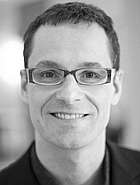
\includegraphics[width=0.5\columnwidth]{media/arthur.jpg}}
\end{center}

\citequotes{Ich möchte steuern, wer welche Aufgabe im Projekt übernimmt und über Problemen informiert sein. Ich möchte jederzeit einsehen können, welcher Anteil der Texte bereits fertig ist.}

Arthur koordiniert als Projektleiter mit allen Beteiligten den Ablauf des Projektes, hat jedoch keinen Einfluss auf die eigentlichen Texte.

\textbf{Organisation, Abstimmung}

Arthur arbeitet auf Seiten der Agentur und stimmt sich über organisatorische Fragen mit allen Beteiligten ab.

\textbf{Werkzeuge und Erfahrung}

Arthur arbeitet vor allem mit \trademark{Word}, \trademark{Excel} und \trademark{PowerPoint}, findet sich aber leicht in anderen Anwendungen zurecht.

\textbf{Anforderungen}

Für Arthur muss das System vor allem immer verfügbar sein, Unterbrechungen im Projektverlauf durch einen Systemausfall sind nicht akzeptabel. Auch ein Datenverlust muss ausgeschlossen sein. Es muss möglich sein alle Daten des Projektes zu exportieren.

\columnbreak

\textbf{Zugang}

Arthur greift von seinem Laptop auf das System zu und verfügt über eine schnelle Internetverbindung.

\textbf{Szenarien}

Arthur legt ein neues Projekt an und fügt Mitarbeiter mit Hilfe ihrer E-Mail-Adressen hinzu. Er kann Mitarbeitern Rollen zuweisen, damit klar ist, welche Aufgabe sie haben. 

Die Rechtsabteilung des Kunden muss die AGB, das Impressum und die Datenschutzbedingungen einer Website abnehmen. Arthur konfiguriert den Workflow im System so, dass diese Texte von allen Mitarbeitern dieser Abteilung freigegeben werden müssen.

Arthur beauftragt ein Lektorat mit der Kontrolle aller Texte. Er konfiguriert den Workflow so, dass Texte erst durch den Kunden einsehbar sind, wenn die Mitarbeiter des Lektorats alle geprüft haben.

Anhand der Aufzeichnungen seit Projektbeginn kann das System für Arthur einen voraussichtlichen Abschlusstermin berechnen. Es ist ersichtlich, dass der Texter für die Erstellung seiner Texte zu lange braucht. Arthur zieht einen Texter aus einem anderen Projekt ab und weist ihn diesem Projekt zu. Das System berechnet mit der zusätzlichen mittleren Arbeitsleistung des neuen Texters ein neues Enddatum, das jetzt Arthurs Vorstellung entspricht.

\end{multicols}

\pagebreak
